\subsection{Utilisation du client}

\subsubsection{Lancement du client}

Le client sert à générer l'interface graphique à l'utilisateur pour lui permettre de jouer. Pour lancer le client, il faut entrer la commande suivante :
\begin{verbatim}
./sh13.exe <server ip address> <server port> <client ip address> <client port> <player name>
\end{verbatim}
Tous les arguments sont obligatoires. L'adresse ip et le port du serveur doivent être ceux utilisés par le serveur lancé. L'adresse ip du client spécifié peut être localhost. Le port client spécifié doit être disponible. Par exemple, les ports 32 001, 32 002, 32 003, etc. Un nom de joueur doit être renseigné.

\subsubsection{Connection au serveur}

Une fois la commande exécutée, une fenêtre graphique s'ouvrira :
\begin{figure}[H]
    \begin{center}
        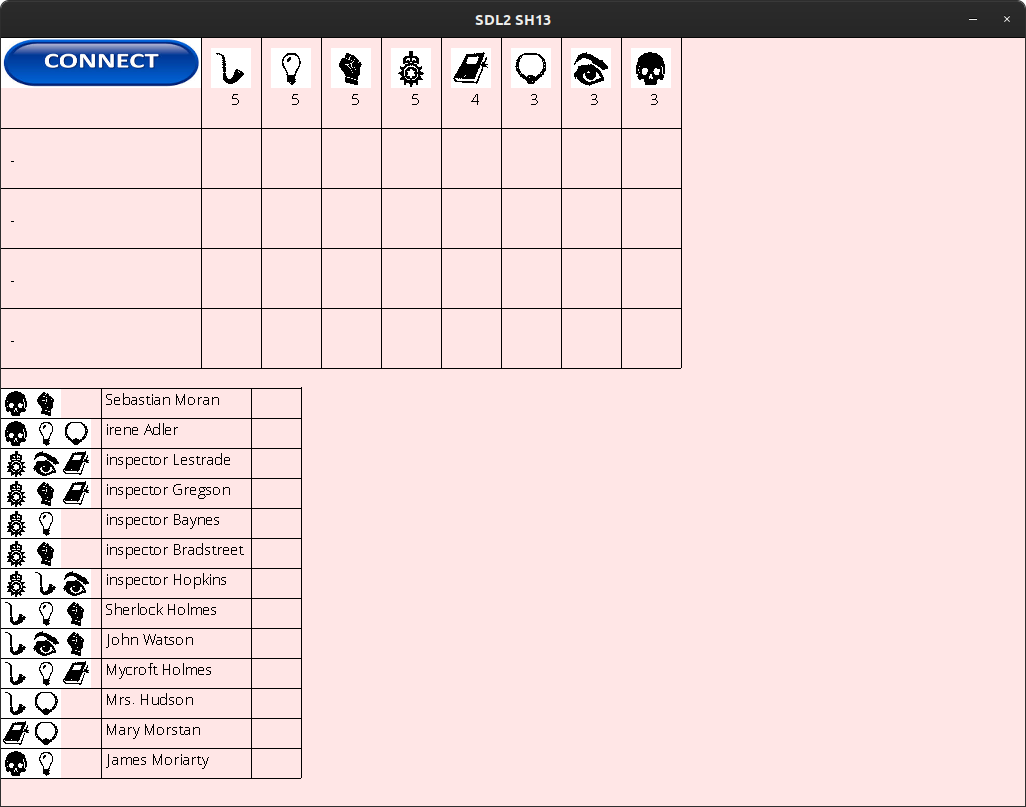
\includegraphics[width=.5\linewidth]{avant_connection.png}
    \end{center}
     \caption{Fenêtre graphique avant connection}
    \label{fig:avant_connection}
\end{figure}
En cliquant sur le bouton <<CONNECT>>, vous aurez accès aux noms des autres joueurs déjà connectés :
\begin{figure}[H]
    \begin{center}
        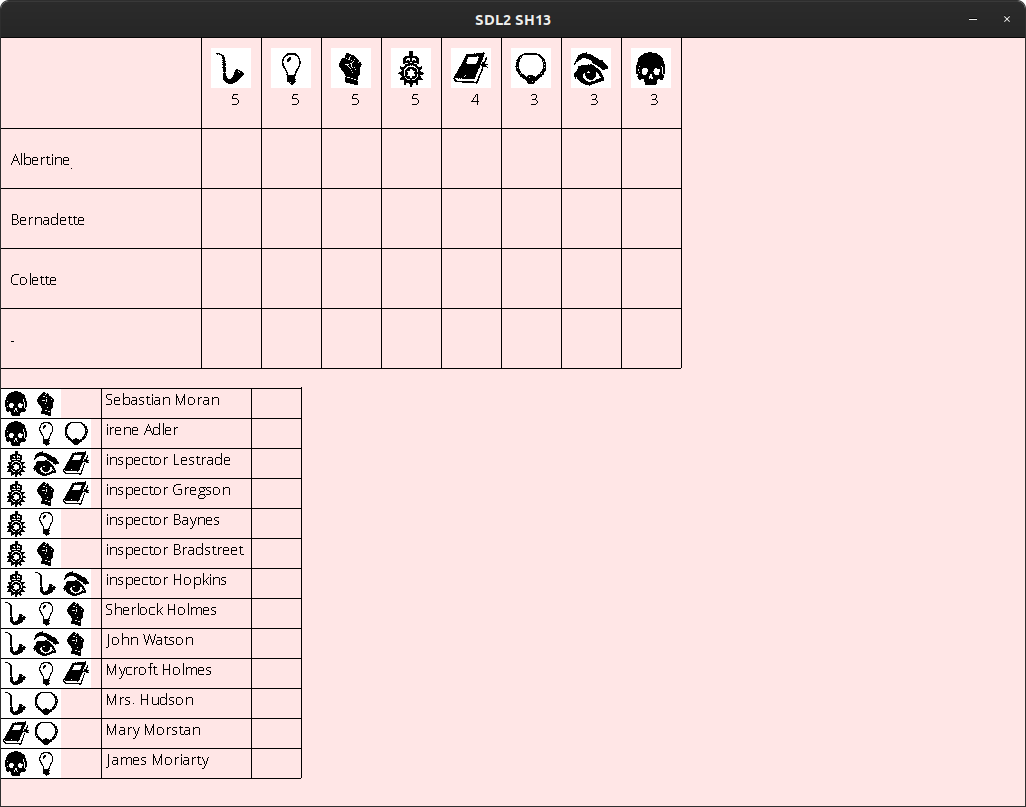
\includegraphics[width=.5\linewidth]{apres_connection.png}
    \end{center}
   	 \caption{Fenêtre graphique après connection}
    \label{fig:après_connection}
\end{figure}
Une fois que le quota de joueurs connectés est atteint, la partie peut commencer !
\begin{figure}[H]
    \begin{center}
        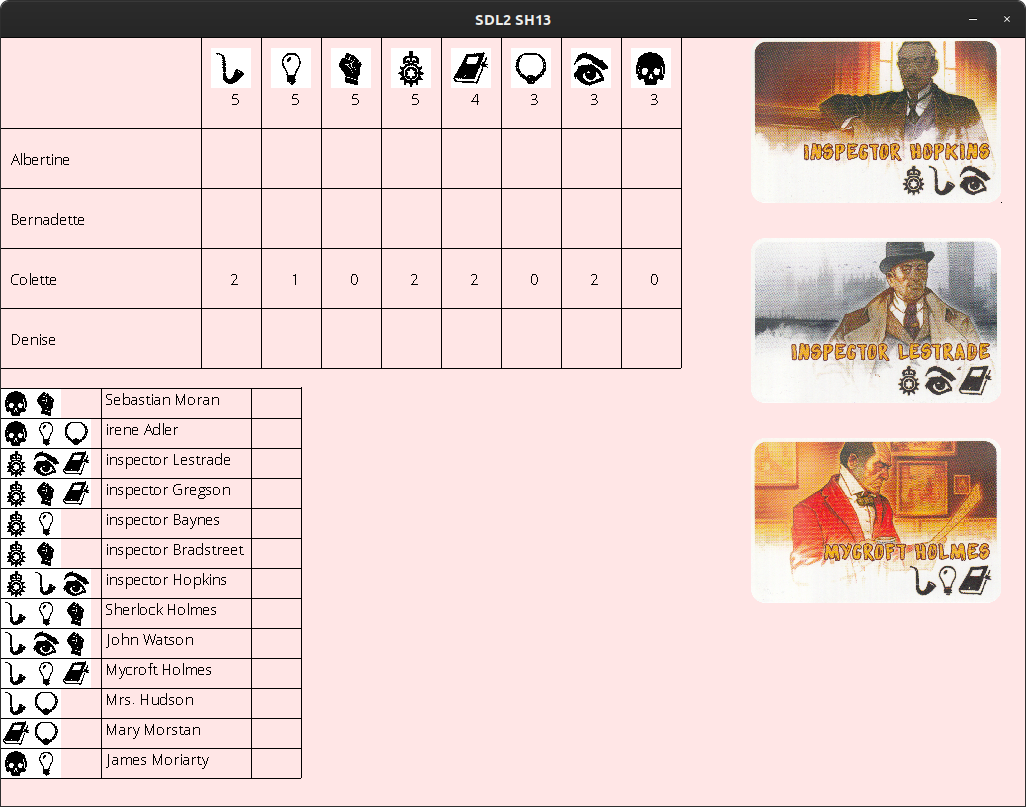
\includegraphics[width=.5\linewidth]{debut.png}
    \end{center}
     \caption{Début de partie}
    \label{fig:debut}
\end{figure}

\subsubsection{Actions disponibles}

Une fois sur la partie lancée, plusieurs actions sont disponibles :
\begin{description}
  \item[Utilisation du mémo] : (figure \ref{fig:memo}) En cliquant dans les cases à côté des noms des différents personnages, vous pouvez indiquer qui vous sembles présent dans les mains des différents joueurs.
  \item[Savoir qui possède un symbole] : (figure \ref{fig:qui_symbole}) En cliquant sur la case du symbole en question et en confirmant son action (en cliquant sur le bouton go), vous pourrez savoir quels joueurs possèdent des personnages liés à ce symbole.
  \item[Savoir combien de fois un joueur possède un symbole] : (figure \ref{fig:combien_symbole}) En cliquant sur la case du symbole en question ainsi que la case du joueur souhaité et enfin en confirmant son action (en cliquant sur le bouton go), vous pourrez savoir combien de personnage sont liés à ce symbole dans la main de l'autre joueur.
  \item[Accuser un des personnages] : (figure \ref{fig:accusation}) En cliquant sur le nom d'un personage et en confirmant son action (en cliquant sur le bouton go), vous lancez une accusation.
\end{description}

\begin{figure}[H]
     \centering
     \begin{subfigure}{.45\linewidth}
       \centering
           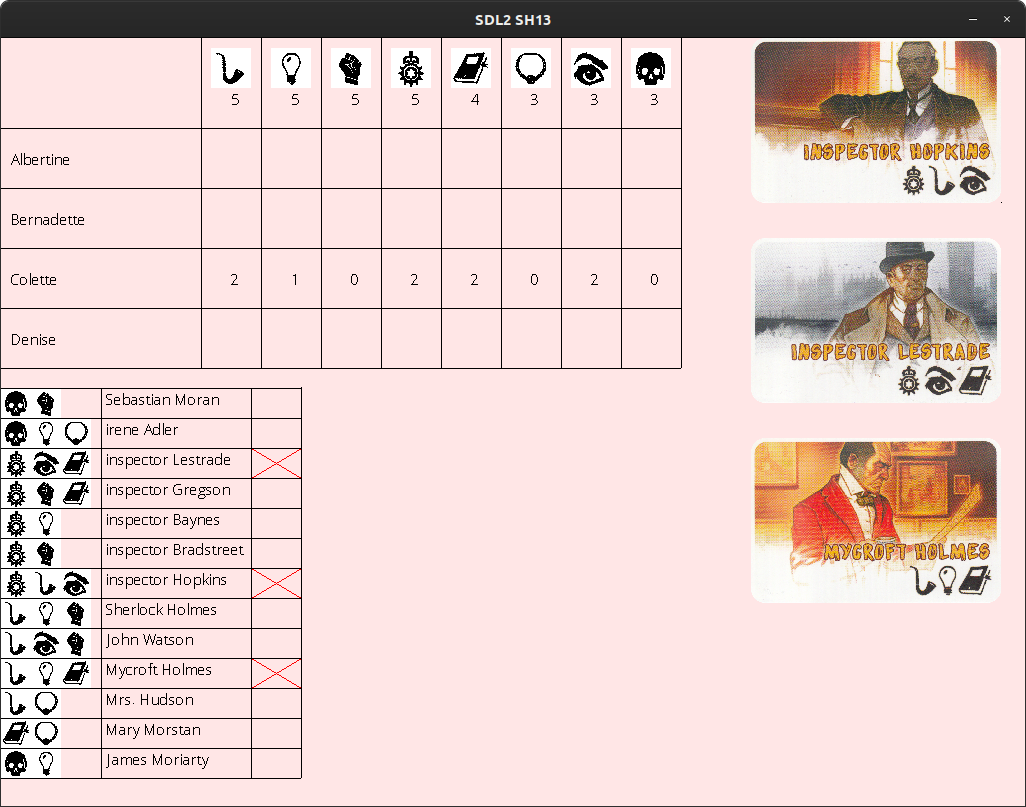
\includegraphics[width=\linewidth]{memo.png}
       \caption{Utilisation du mémo}
       \label{fig:memo}
     \end{subfigure}
     \hspace{1em}
     \begin{subfigure}{.45\linewidth}
	  \centering
       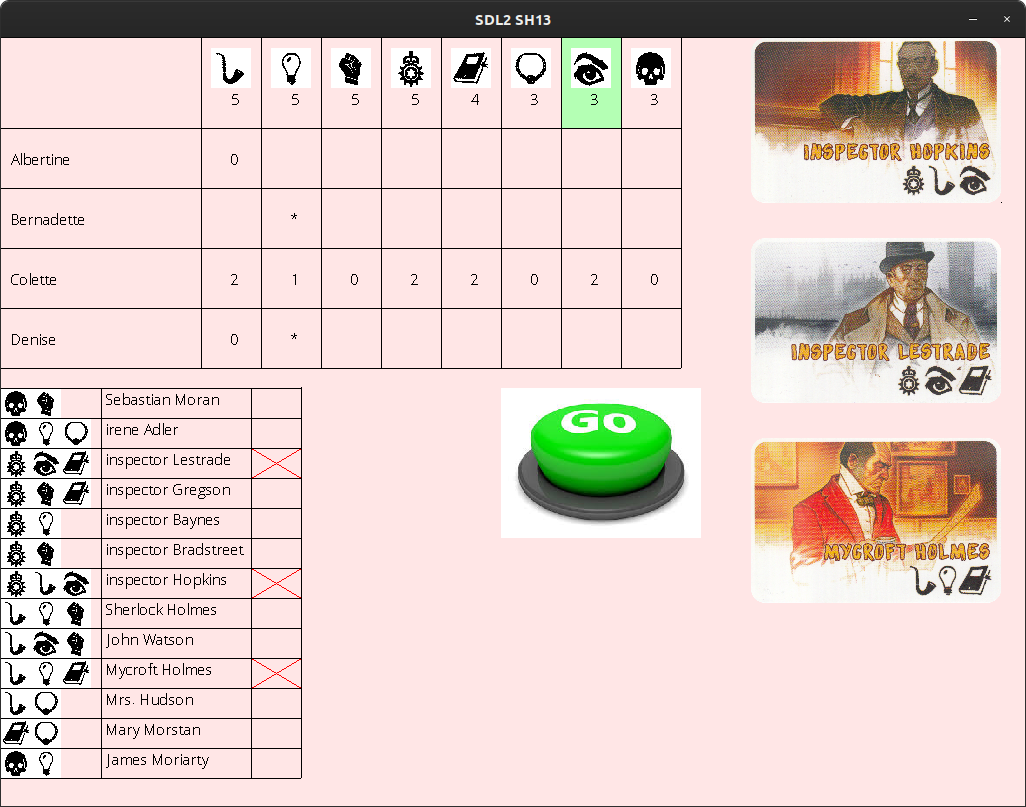
\includegraphics[width=\linewidth]{qui_symbole.png}
       \caption{Savoir qui possède un symbole}
       \label{fig:qui_symbole}
     \end{subfigure}
     \hspace{1em}
     \begin{subfigure}{.45\linewidth}
         \centering
         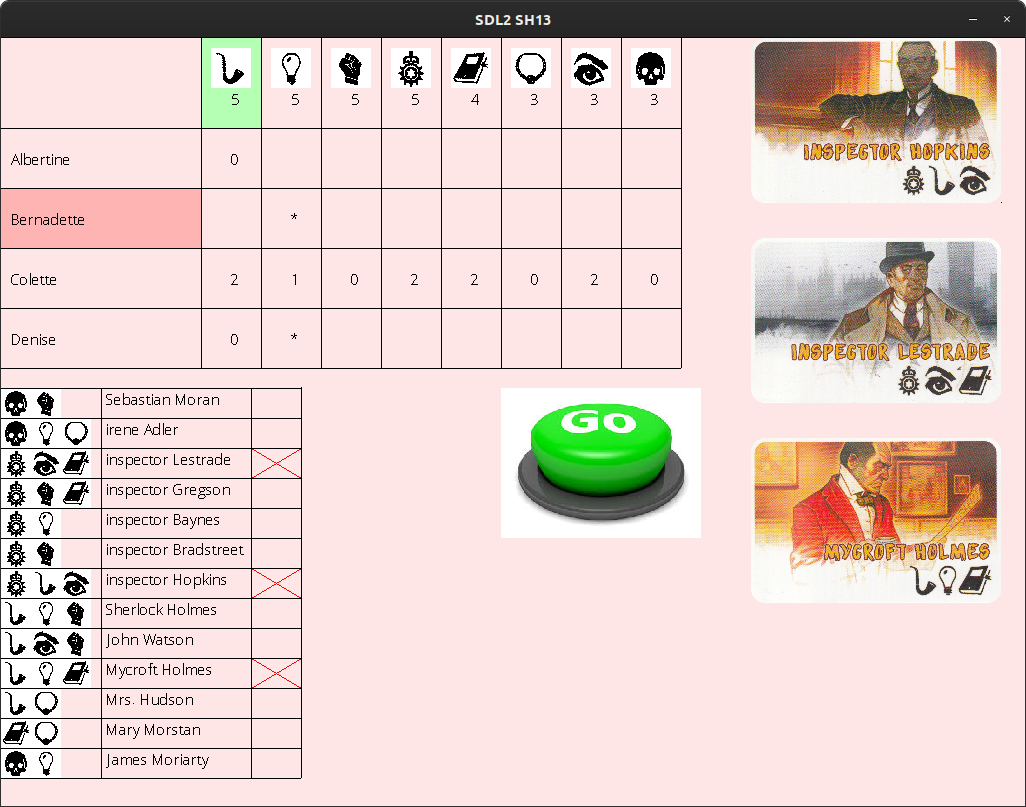
\includegraphics[width=\linewidth]{combien_symbole.png}
        \caption{Savoir combien de fois un joueur possède un symbole}
       \label{fig:combien_symbole}
     \end{subfigure}
     \hspace{1em}
     \begin{subfigure}{.45\linewidth}
	 \centering
           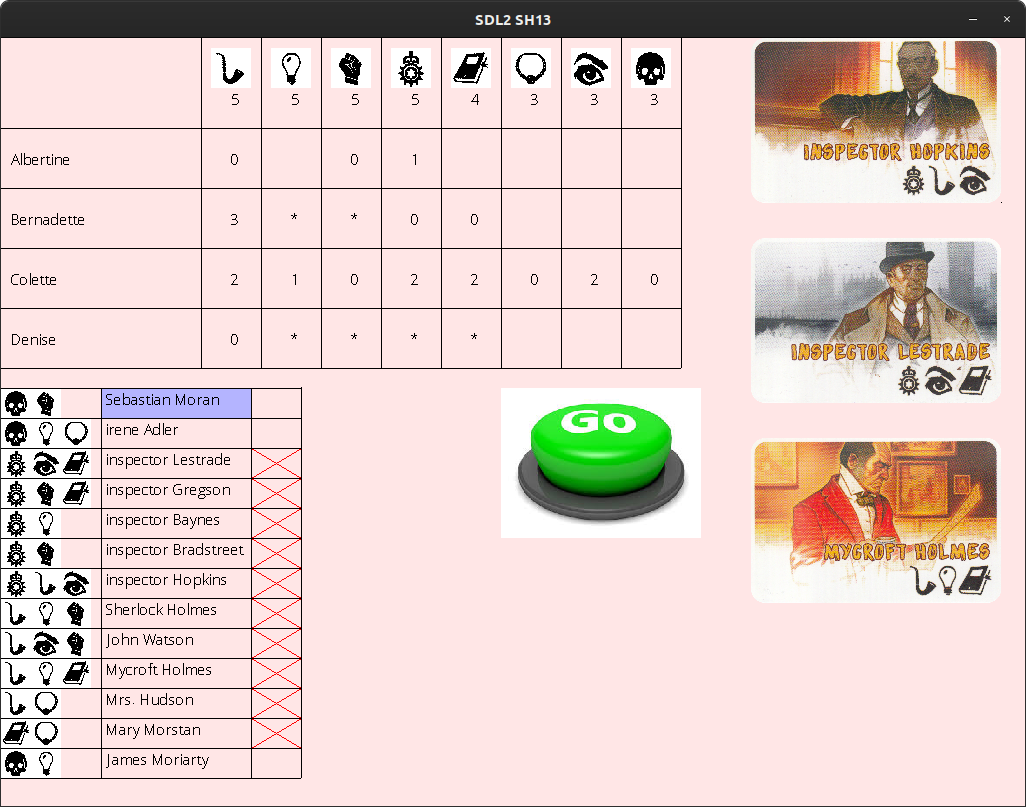
\includegraphics[width=\linewidth]{accusation.png}
      	   \caption{Accuser un des personnages}
       \label{fig:accusation}
     \end{subfigure}
     \caption{Captures des différentes actions}
\end{figure}

Pour ces trois dernières actions, il est nécessaire de cliquer sur le bouton go (et donc mettre fin à son tour) pour les valider. Pour annuler la sélection, il suffit de cliquer en dehors de tout encart.

Enfin, une fausse accusation entraîne la défaite du joueur tandis que la bonne accusation apporte sa victoire.

\begin{figure}[H]
     \centering
     \begin{subfigure}{.45\linewidth}
         \centering
         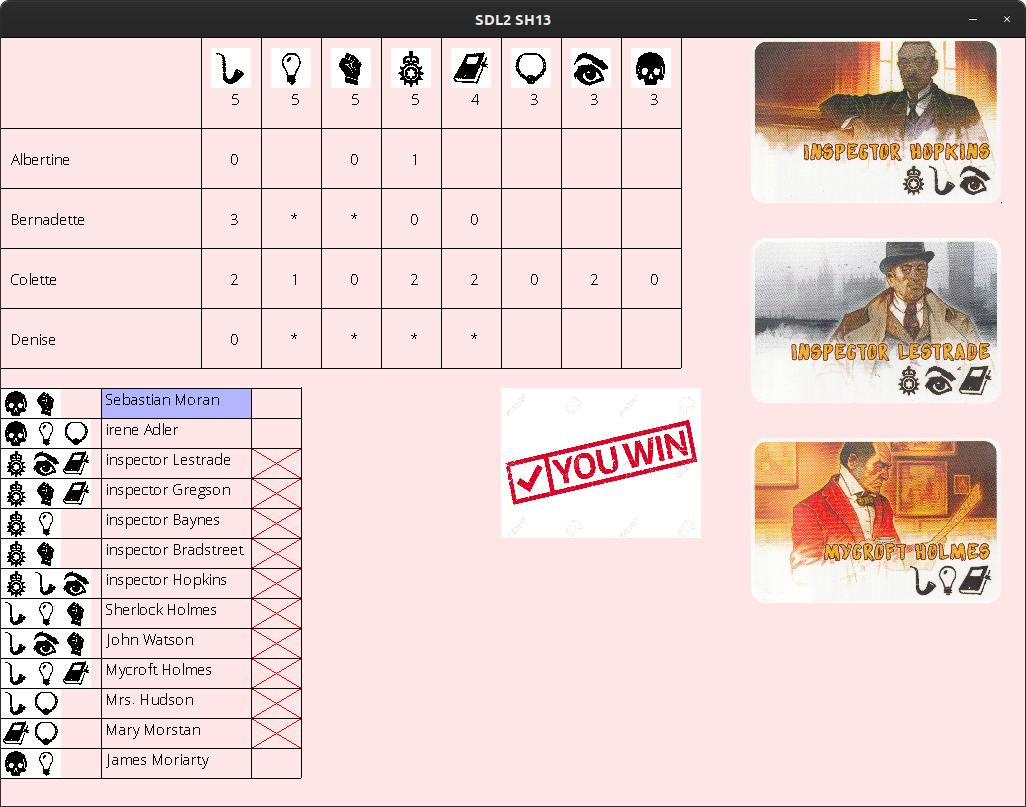
\includegraphics[width=\linewidth]{perdre.png}
         \caption{Victoire}
		\label{fig:victoire}
     \end{subfigure}
     \hspace{1em}
     \begin{subfigure}{.45\linewidth}
         \centering
         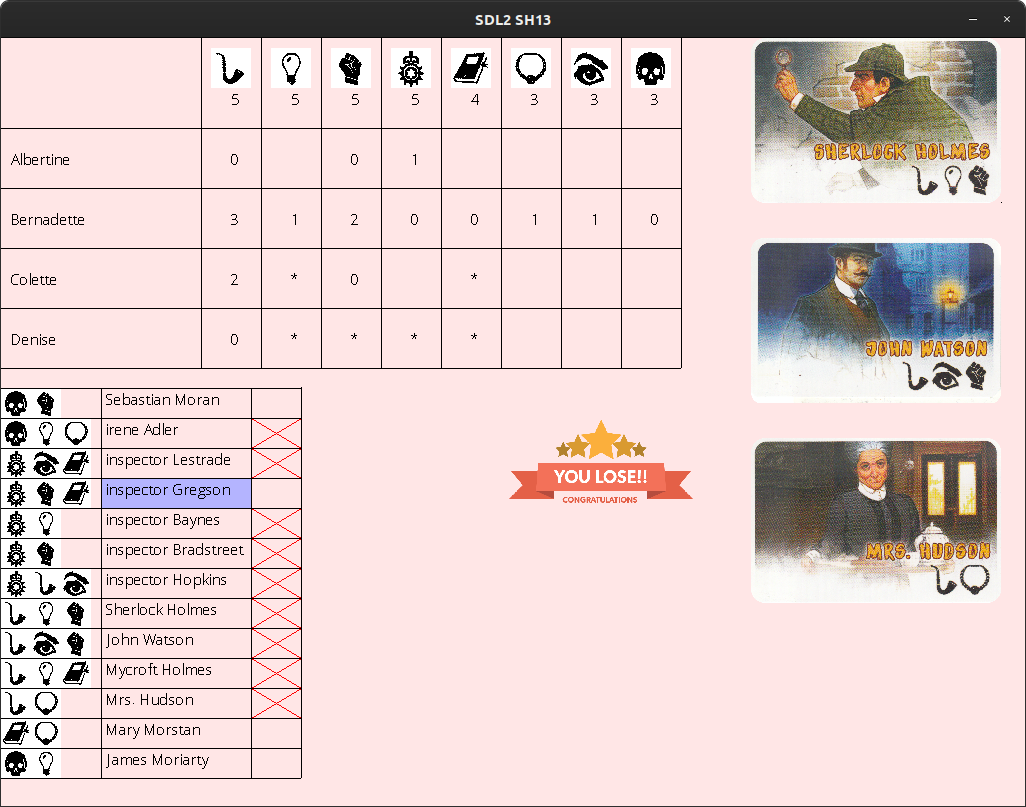
\includegraphics[width=\linewidth]{gagner.png}
         \caption{Défaite}
		\label{fig:defaite}
     \end{subfigure}
\end{figure}

\subsubsection{Fermeture du client}

Pour mettre fin au programme, il suffit de cliquer sur la croix de fermeture de la fenêtre graphique ou de sélectionner sa console et appuyer sur les touches \verb|Ctrl + C|.
